\section{Task 1: Preliminary Data Analysis}
\label{sec:task1}

Before fitting any model, the five signals were explored to understand their range, shape and dependencies. Table~\ref{tab:summary} gives the summary statistics, produced by the \texttt{summary()}, \texttt{sd()} and skewness lines of the Task~1 script (Appendix~\ref{app:task1}).

\begin{table}[H]
\centering
\caption{Summary statistics of the five signals ($n=10{,}000$).}
\label{tab:summary}
\begin{tabular}{lrrrrrrr}
\toprule
Signal & Min & Q1 & Median & Mean & Q3 & Max & Skewness \\
\midrule
$x_1$ CPU      & 1.00  & 2.72  & 4.45  & 4.46  & 6.18  & 8.00  & 0.03 \\
$x_2$ Memory   & 2.00  & 3.78  & 5.54  & 5.53  & 7.30  & 9.00  & $-0.02$ \\
$x_3$ Disk I/O & $-0.78$ & 3.99 & 5.01 & 5.00 & 6.01 & 11.72 & 0.01 \\
$x_4$ Network  & 0.00  & 0.87  & 2.08  & 3.00  & 4.14  & 27.36 & 1.94 \\
$y$ Power      & 121.7 & 507.1 & 828.3 & 1084.1 & 1375.9 & 15241.3 & 2.71 \\
\bottomrule
\end{tabular}
\end{table}

\subsection{Task 1.1: Time series plots}
Figure~\ref{fig:ts} plots every signal against time over the full 1000\,s. With 10{,}000 points the plots turn into dense bands. They still show that no signal has a trend, a level shift or a change in spread over time: all five are stationary. Disk I/O ($x_3$) varies around a level of about 5. Network traffic ($x_4$) sits near zero with frequent short spikes. Power ($y$) shows the same spiky shape, with a few very large peaks of up to about 15{,}000\,W.

\begin{figure}[H]
\centering
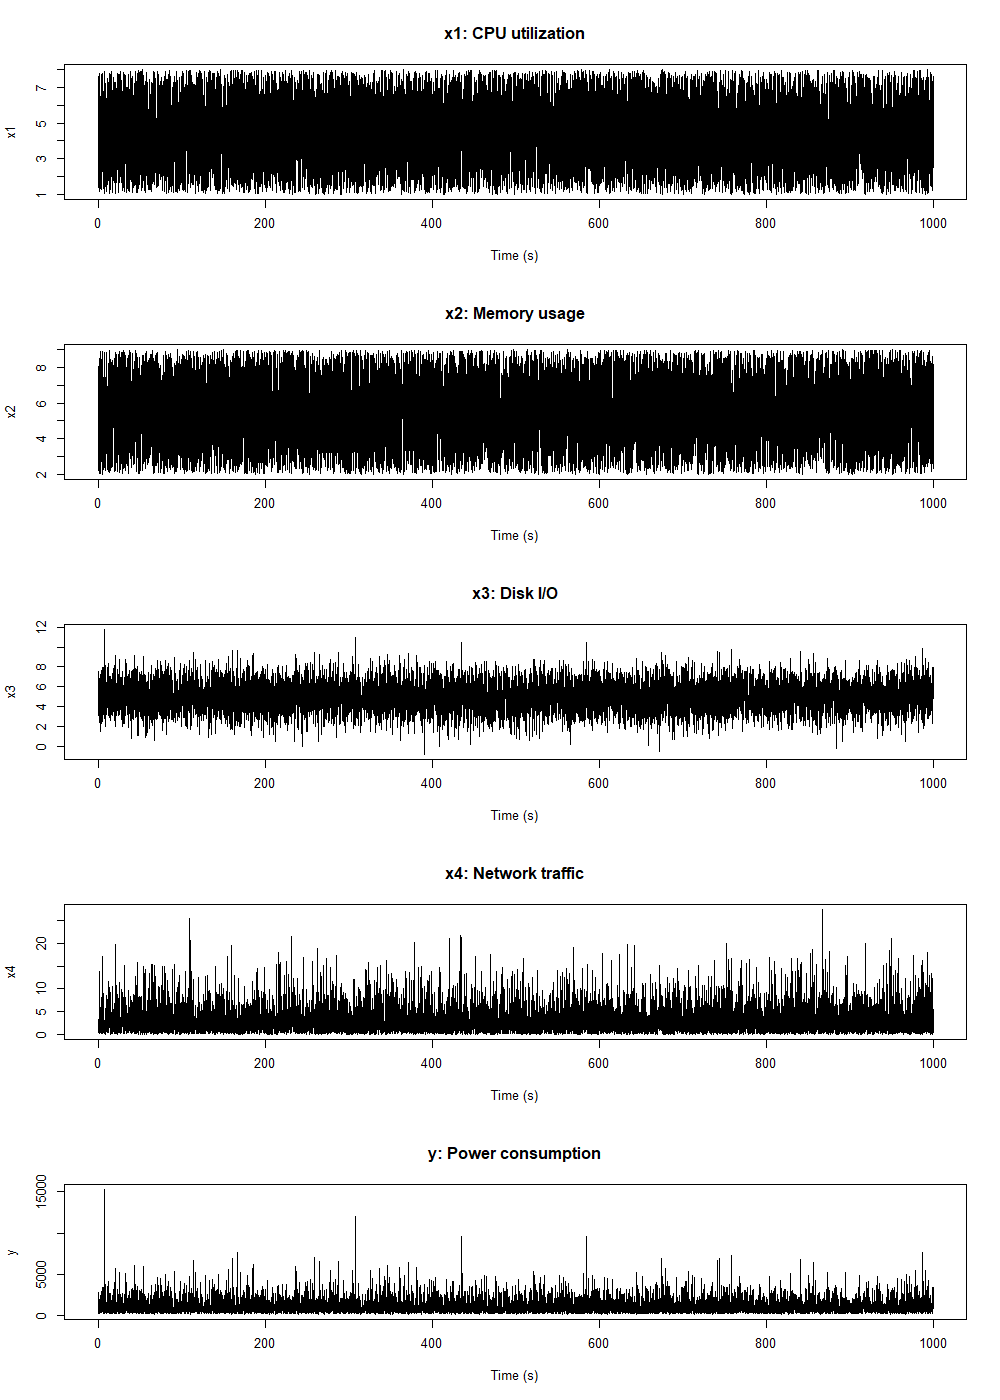
\includegraphics[width=0.78\textwidth]{fig1_time_series.png}
\caption{Time series of the four inputs and the output power over the full 1000\,s record.}
\label{fig:ts}
\end{figure}

Figure~\ref{fig:tszoom} zooms in on the first 20\,s (200 samples) so that single samples can be seen. Neighbouring samples are not similar: each value looks like a fresh random draw, with no cycles or smooth movements. The lag-1 autocorrelation of every signal is between $-0.012$ and $0.011$, which confirms this. The samples can therefore be treated as independent observations, which the regression assumption of i.i.d.\ errors needs. The time stamp carries no useful information for modelling. The plot also shows that the large power spike at about 7\,s happens at the same time as a spike in disk I/O, which is a first hint that $y$ depends strongly on $x_3$.

\begin{figure}[H]
\centering
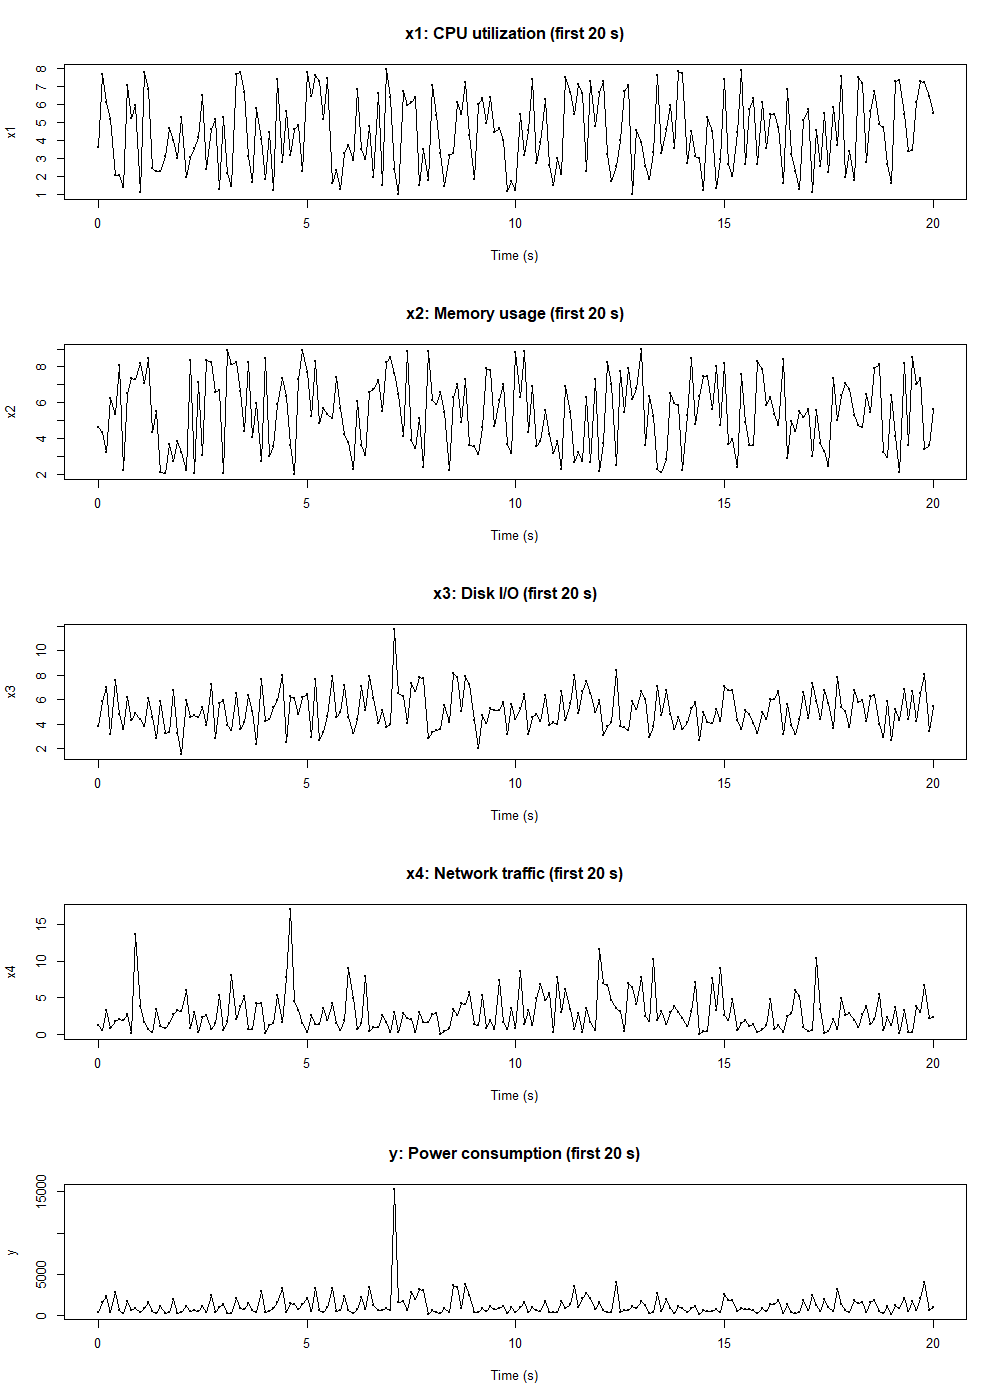
\includegraphics[width=0.78\textwidth]{fig1b_time_series_zoom.png}
\caption{Zoomed time series of the first 20\,s (200 samples).}
\label{fig:tszoom}
\end{figure}

\subsection{Task 1.2: Distribution of each signal}
Figure~\ref{fig:dist} shows a histogram of each signal with a kernel density curve. The four inputs have clearly different shapes:
\begin{itemize}
  \item $x_1$ (CPU) and $x_2$ (memory) are flat between about 1--8 and 2--9. They look \textbf{uniformly distributed}, and the dips at the edges of the density curve are only a smoothing effect.
  \item $x_3$ (disk I/O) is bell-shaped and symmetric around 5 (skewness 0.01). It looks \textbf{normally distributed}, with standard deviation about 1.5.
  \item $x_4$ (network) is strongly \textbf{right-skewed} (skewness 1.94). Its mean (3.0) equals its standard deviation (3.0) and it never goes below zero, which matches an exponential distribution.
  \item $y$ (power) is also strongly right-skewed (skewness 2.71) with a long upper tail.
\end{itemize}
The output is skewed even though $x_3$ is symmetric, which suggests that $y$ depends on a high power of an input: raising a symmetric variable to the fourth power stretches its upper tail.

\begin{figure}[H]
\centering
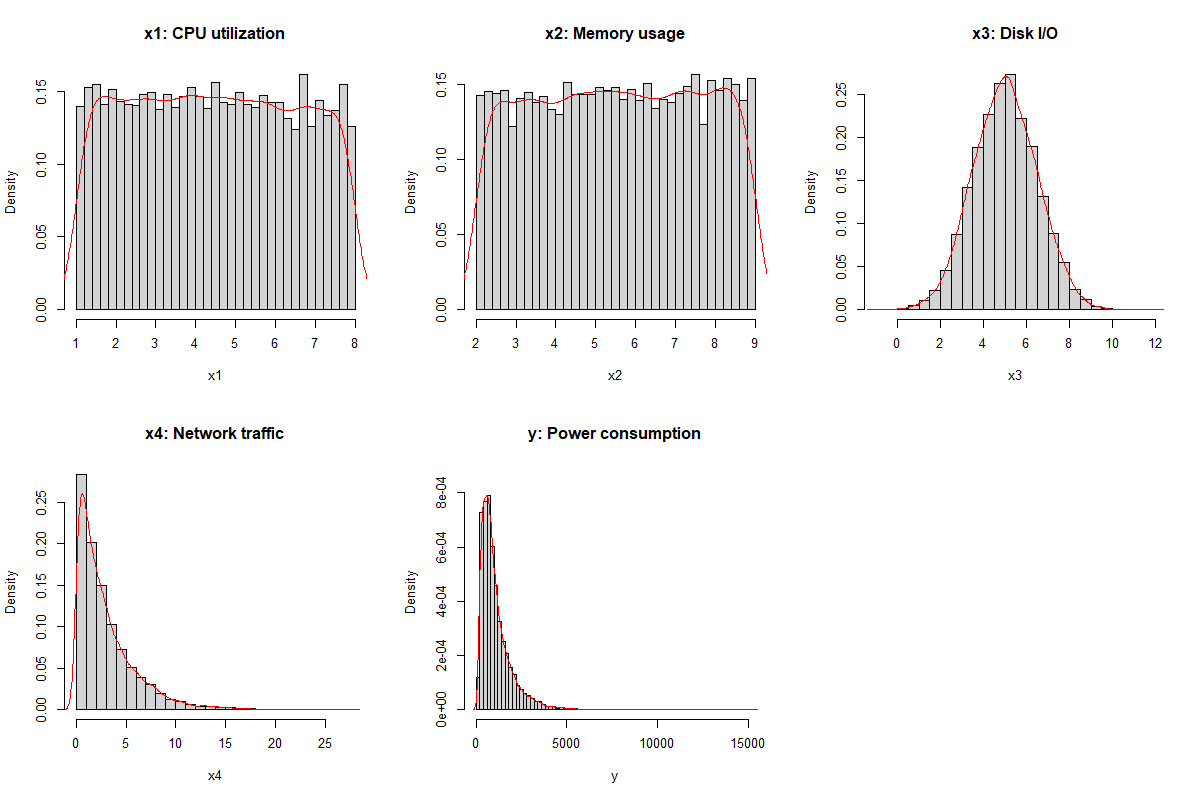
\includegraphics[width=0.95\textwidth]{fig2_distributions.png}
\caption{Histograms with kernel density estimates (red) for each signal.}
\label{fig:dist}
\end{figure}

\subsection{Task 1.3: Correlation and scatter plots}
Table~\ref{tab:cor} and Figure~\ref{fig:corr} give the correlation between all pairs of signals. The inputs are almost uncorrelated with each other ($|r|\le0.023$), so there is no multicollinearity and the effect of each input can be estimated separately. Against the output:
\begin{itemize}
  \item $x_3$ has a strong positive correlation ($r=0.851$). Its Spearman rank correlation is even higher (0.931), which shows that the relationship is monotonic but \emph{not} linear.
  \item $x_1$ has a weak positive correlation ($r=0.174$, Spearman 0.291).
  \item $x_2$ ($r=-0.014$) and $x_4$ ($r=0.010$) show no visible correlation.
\end{itemize}

\begin{table}[H]
\centering
\caption{Correlation of each input with the output $y$.}
\label{tab:cor}
\begin{tabular}{lcccc}
\toprule
 & $x_1$ & $x_2$ & $x_3$ & $x_4$ \\
\midrule
Pearson $r$ with $y$   & 0.174 & $-0.014$ & 0.851 & 0.010 \\
Spearman $\rho$ with $y$ & 0.291 & $-0.012$ & 0.931 & 0.016 \\
\bottomrule
\end{tabular}
\end{table}

\begin{figure}[H]
\centering
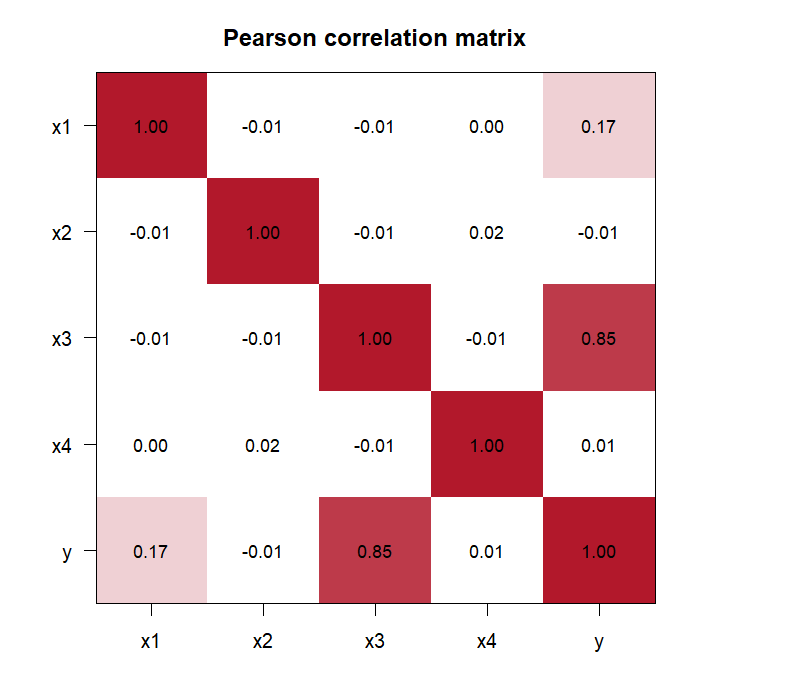
\includegraphics[width=0.6\textwidth]{fig3a_correlation.png}
\caption{Pearson correlation matrix of all signals.}
\label{fig:corr}
\end{figure}

The scatter plots in Figure~\ref{fig:scatter} show the shape of each relationship. The plot of $y$ against $x_3$ shows a clear, tight, upward curve that gets steeper as $x_3$ grows, which is typical of a high-order polynomial term. The plot against $x_1$ shows a lower boundary of the point cloud that rises with $x_1$, so $x_1$ has a smaller non-linear effect that is hidden by the spread caused by $x_3$. The plots against $x_2$ and $x_4$ have flat LOWESS lines.

A low correlation does not prove that an input has no effect. The spread in $y$ caused by $x_3$ (standard deviation 884\,W) is so large that a small linear effect of $x_4$ cannot be seen in a two-variable plot. This is why the models must be compared with all inputs together, as in Task~2.

\begin{figure}[H]
\centering
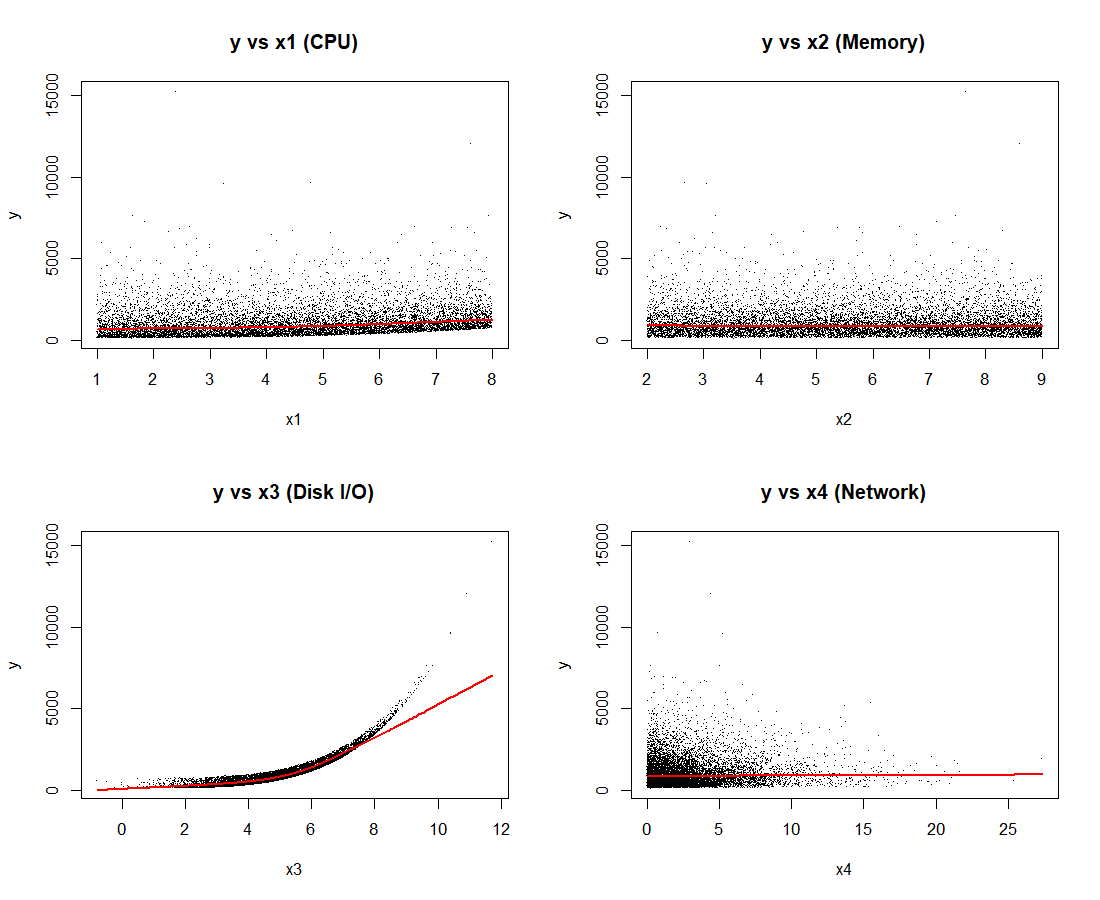
\includegraphics[width=0.85\textwidth]{fig3_scatter.png}
\caption{Scatter plots of the output power against each input, with LOWESS curves (red).}
\label{fig:scatter}
\end{figure}

\subsection{Baseline linear model}
As a reference, a linear model with all four inputs was fitted with \texttt{lm()}. It explains 75.9\% of the variance ($R^2=0.7587$) with a residual standard error of 434.1\,W. $x_1$, $x_3$ and $x_4$ are significant ($p<0.001$), but $x_2$ is not ($p=0.46$). The residual plots in Figure~\ref{fig:linres} show that the linear model is not adequate. The residuals form a curved pattern against the fitted values, and the Q-Q plot bends sharply upwards in the right tail. Both signs mean that the true relationship is non-linear, which supports using the polynomial models of Task~2.

\begin{figure}[H]
\centering
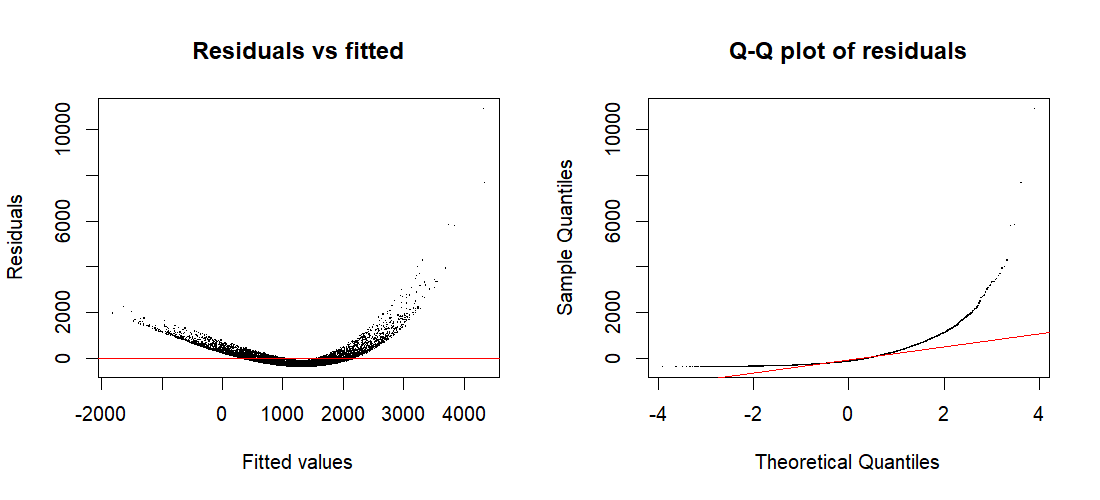
\includegraphics[width=0.85\textwidth]{fig4_linear_residuals.png}
\caption{Residuals vs fitted values and normal Q-Q plot for the baseline linear model.}
\label{fig:linres}
\end{figure}
